\documentclass[12pt]{article}
\usepackage{setspace}   % double spacing
\usepackage{geometry}   % margins 
\usepackage{hyperref}   % hyperlinks
% \usepackage{mathptmx}   % times new roman
\usepackage{tocloft}    % table of contents
\usepackage{graphicx}   % graphics
\usepackage{placeins}   % manage placement of figures
\usepackage[
    backend=bibtex,
    style=ieee,
]{biblatex}
\addbibresource{refs.bib}
% ========================================== %
% document options
\setstretch{2} % double spacing
\raggedright
\geometry{ 
    a4paper,
    margin=1in,
    lmargin=1.5in
}

% hyperlinks for toc
\usepackage{xcolor}
\hypersetup{
    colorlinks,
    linkcolor={red!50!black},
    citecolor={blue!50!black},
    urlcolor={blue!80!black}
}
% ========================================== %
% section notations
\renewcommand*\contentsname{ 
    {\MakeUppercase{Table of Contents}} 
}
\renewcommand*\listfigurename{ 
    {
        \section*{LIST OF FIGURES}
        \addcontentsline{toc}{section}{LIST OF FIGURES}
    } 
}
\renewcommand*\listtablename{
    {
        \section*{{LIST OF TABLES}}
        \addcontentsline{toc}{section}{LIST OF TABLES}
    } 
}
% ========================================== %
% custom variables
\newcommand{\thesistitle}{
    {\Large A comparative study of texture analysis methods on
ant head images}
}
% \newcommand{\toppage}{\vspace*{0.1in}}
% ========================================== %

\begin{document}
\pagenumbering{roman}
% ========================================== %
% thesis premable page
\begin{center}
    \textbf{\MakeUppercase{\thesistitle}}
    \vspace{1in}

    A Thesis Presented to

    The Faculty of the Computer Science Department
    \vspace{1in}

    by
    \vspace{0.5in}

    Noah Gardner
    \vspace{1in}

    In Partial Fulfillment

    of Requirements for the Degree

    Master of Science in Computer Science

    \vspace{1in}
    Kennesaw State University

    May 2022
\end{center}
\thispagestyle{empty}
\newpage

% ========================================== %
% agreement
\noindent In presenting this thesis as a partial fulfillment of the requirements
for an advanced degree from Kennesaw State University, I agree that the
university library shall make it available for inspection and circulation in
accordance with its regulations governing materials of this type. I agree that
permission to copy from, or to publish, this thesis may be granted by the
professor under whose direction it was written, or, in his absence, by the dean
of the appropriate school when such copying or publication is solely for
scholarly purposes and does not involve potential financial gain. It is
understood that any copying from or publication of, this thesis which involves
potential financial gain will not be allowed without written permission.
\vspace{2in}

\def\dotsign{\xleaders\hbox to .2em{\d{}}\hfill\d{}}
\begin{center}
    \makebox[.5\linewidth][r]\dotsign\smallskip\\
    Noah Gardner
\end{center}
\newpage

% ========================================== %
% notice to borrowers
\begin{center}
    \textbf{\underline{Notice to Borrowers}}
\end{center}
\vspace{0.5in}

\noindent Unpublished theses deposited in the Library of Kennesaw State
University must be used only in accordance with the stipulations prescribed by
the author in the preceding statement.
\vspace{0.5in}

\noindent The author of this thesis is:
\begin{center}
    Noah Gardner

    1100 S Marietta Parkway

    Marietta, GA 30060
\end{center}

\noindent The director of this thesis is:
\begin{center}
    Chih-Cheng Hung

    1100 S Marietta Parkway

    Marietta, GA 30060
\end{center}
\vspace{0.5in}

\noindent Users of this thesis not regularly enrolled as students at Kennesaw
State University are required to attest acceptance of the preceding stipulations
by signing below. Libraries borrowing this thesis for the use of their patrons
are required to see that each user records here the information requested.
\vspace{0.3in}

\noindent
Name of user \hspace{0.2in} Address \hspace{0.2in} Date \hspace{0.2in} Type of
use (examination only or copying)
\newpage

% ========================================== %
% abstract preamble page title page
\begin{center}
    \textbf{\MakeUppercase{\thesistitle}}
    \vspace{1in}

    An Abstract of

    A Thesis Presented to

    The Faculty of the Computer Science Department
    \vspace{1in}

    by
    \vspace{0.5in}

    Noah Gardner
    \vspace{1in}

    In Partial Fulfillment

    of Requirements for the Degree

    Master of Science in Computer Science

    \vspace{1in}
    Kennesaw State University

    May 2022
\end{center}
\newpage

% ========================================== %
% abstract page
\begin{center}
    \section*{ABSTRACT}
    \addcontentsline{toc}{section}{ABSTRACT}
\end{center}
\vspace{0.5in}

\noindent There is a large variety of ant species, and most species are diverse
in terms of size, shape, behaviors, and especially skin (cuticle) textures.
However, the significance of ant cuticle texture is not widely researched. Ant
cuticle texture presumably provides some type of function, and therefore is
useful to research for ecological applications and bioinspired designs. This
research employs modern machine learning methods such as texture analysis and
deep machine learning to automatically group similar ant species based on
morphological traits. We provide a comparative study of the performance of
modern texture analysis methods on ant head images. We evaluate the results of
the classification methods with modern visualization techniques.

\newpage

% ========================================== %
% advisor preamble
\begin{center}
    \textbf{\MakeUppercase{\thesistitle}}
    \vspace{1in}

    A Thesis Presented to

    The Faculty of the Computer Science Department
    \vspace{1in}

    by
    \vspace{0.5in}

    Noah Gardner
    \vspace{1in}

    In Partial Fulfillment

    of Requirements for the Degree

    Master of Science in Computer Science
    \vspace{0.5in}

    Advisor: Dr. Chih-Cheng Hung
    \vspace{0.5in}

    Kennesaw State University

    May 2022
\end{center}
\newpage

% ========================================== %
% dedication page
\vspace*{\fill}
\begin{center}
    \textit{To my family}
\end{center}
\vspace*{\fill}
\newpage

% ========================================== %
% quote page
\vspace*{2in}
Never fail to have this attitude of mind, go forward without hurry, learn the
essence of things through frequent experiences, taking advantage of every
occasion. Fight against all kinds of people and be aware of their mind. Follow a
road that is a thousand leagues long one step at a time. Be without haste and be
convinced that all these practices are the duty of a bushi. Be victorious today
over what you were yesterday; tomorrow be victorious over your clumsiness and
then also over your skill.

\vspace{0.5in}
\hspace*{\fill} Miyamoto Musashi \footnote{Miyamoto Musashi, The Book of Five
    Rings}
\newpage

% ========================================== %
% acknowledgements page
\begin{center}
    \section*{ACKNOWLEDGEMENTS}
    \addcontentsline{toc}{section}{ACKNOWLEDGEMENTS}
\end{center}
\vspace{0.5in}

I would have given up a long time ago without the support of my family. So, I
would like to thank my loving family for their support throughout the completion
of my graduate degree. I would also like to thank Dr. Chih-Cheng Hung for his
mentorship for my thesis and for his guidance in my other research projects. I
would like to thank Anthony Phan, my undergraduate assistant and friend for his
help in running the experiments. Next, I would like to thank Dr. Zhiling Long
for his insights for machine learning and texture analysis. I would like to
thank John Paul Hellenbrand, his advisor Dr. Clint Penick, and their lab for
providing the project and dataset. Finally, I would like to thank Dr. Coskun
Tekes for providing the Lambda Labs GPU server for my experiments.
\newpage

% ========================================== %
% table of contents
\begin{center}
    \tableofcontents
\end{center}
\newpage

% ========================================== %
% list of figures
\begin{center}
    \listoffigures
\end{center}
\newpage

% ========================================== %
% list of tables 
\begin{center}
    \listoftables
\end{center}
\newpage

% ========================================== %
% begin content
\pagenumbering{arabic}
\setlength{\parskip}{\baselineskip}

% ========================================== %
% chapter 1 - introduction
\section{CHAPTER 1: INTRODUCTION}
\subsection{Introduction}

Insects comprise over half of the world's animal biodiversity
\cite{tihelka_evolution_2021}. Insects are vital to many ecosystem functions,
including nutrient recycling, plant propagation, and maintenance of plant and
animal communities \cite{gullan_insects_2009, berenbaum_bugs_1996}. As
technology advances, systems which can automatically analyze insect-based
information are growing in demand by biologists \cite{hassan_advances_2014}. For
example, automatic insect identification systems can be applied to conserve
natural ecosystems, to prevent commercial loss, and to support the study of
insect-related diseases \cite{xia_insect_2018, kaloudis_insect_2005,
    thenmozhi_crop_2019}.

Due to the extensive number of insect species, manual exploration of
insect-based information is difficult and often requires specialized expertise.
Therefore, automated entomology is gaining attraction by both biologists and
computer scientists and is expected to be a major contribution to the future of
insect-based research \cite{martineau_survey_2017}. One of the most commonly
used data types for insect analysis is image data. To develop an image-based
system for insect analysis, we can take advantage of existing work in general
image processing and texture analysis methods.

Ants are highly diverse, fill many ecological niches, and thus are a major topic
of interest \cite{sosiak_multidimensional_2021}. In this work, we explore
automated entomology specifically for ants in order to support ant-based
ecological research. Although there is some work regarding grouping ants into
categories of similar exoskeleton texture (\textit{cuticle}), automated
categorization has yet to become an active area of research. In general, the
goal of automated insect classification methods is species indentification -
\textit{i.e.} the identification of species from a set of observations. Due to
the large number of different ant species, large scale ant species
indentification with standard classification methods is not feasible. Therefore,
we must simplify the problem by either other classifying a certain subset of ant
species or by applying categories to the entire set of ant species.

In many texture analysis methods, the general goal is to automatically
categorize an object into a set of objects with similar texture-based features.
The approach of texture analysis to categorize similarly texture-based objects
corresponds well to the demands of ant identification. Texture analysis has
shown promising results in related fields, such as plant identification
\cite{boudra_plant_2018}. With modern texture analysis methods, the
categorization of ants can be automated and the results can be used to study the
influence of cuticle texture on ant ecology.

\subsection{Research Question}

The overarching question that we wish to address by beginning this research is:
\textit{how does the texture of ant cuticle affect the ant ecology}? However, to
even begin contemplating this question requires a substantial amount of
preliminiary research. One point that is necessary to begin this research is to
create a method of group ants by texture. Additionally, due to the sheer number
of ant species, an automated effort is necessary to group similar ant species.
Therefore, we start our endeavor with a more straightforward research question:
\textit{are texture analysis methods able to group similar ant species}? By the
end of this research, we answer this question by demonstrating a variety of
texture analysis methods and comparing their results on a custom dataset.

\subsection{Proposed Approach}

\begin{figure}
    \centering
    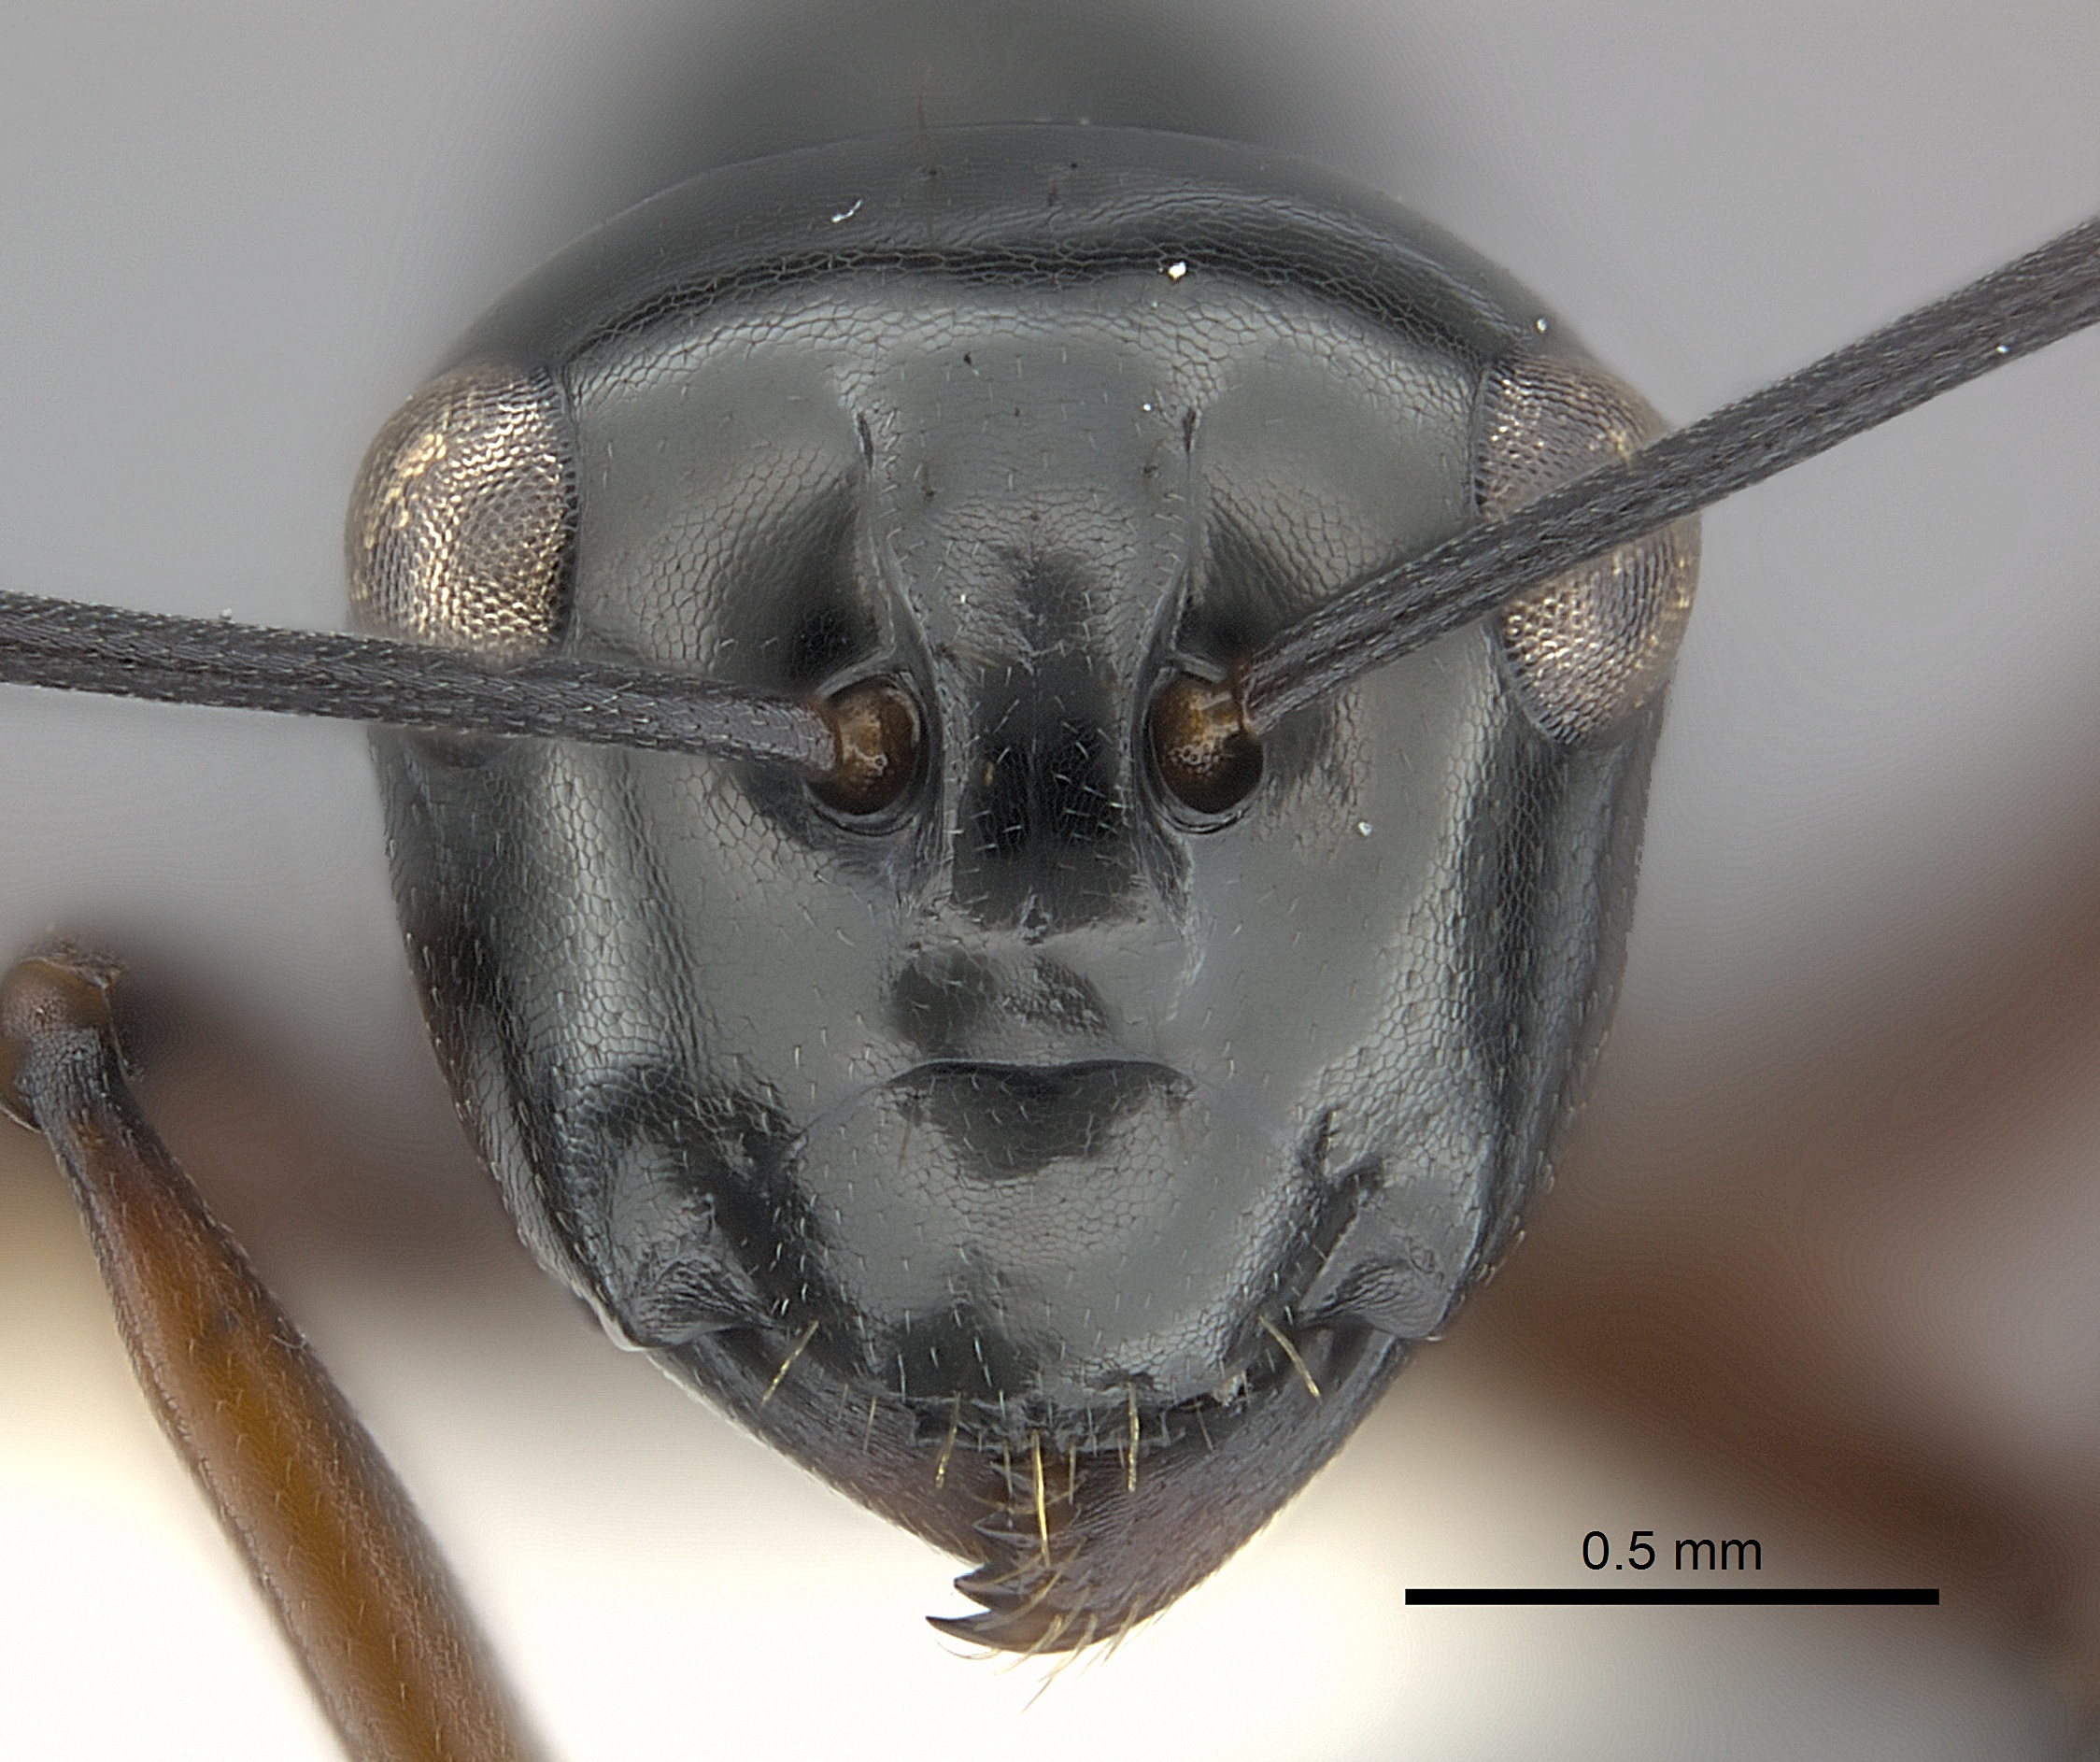
\includegraphics[width=0.8\textwidth]{assets/images/CASENT0217419.jpg}
    \caption{ An example ant head image from AntWeb of species
        \textit{Polyrhachis abbreviata}.
        \href{https://www.antweb.org/bigPicture.do?name=casent0217419&shot=h&number=1}{CASENT0217419}
        by \href{https://www.antweb.org/artist.do?id=92}{Estella Ortega}, from
        \href{https://www.antweb.org}{AntWeb}, is licensed under
        \href{https://creativecommons.org/licenses/by/4.0/}{CC BY 4.0}.}
    \label{fig:CASENT0217419}
\end{figure}

In order to group similar ant species, we require mostly uniform images that
depict the texture of the ant cuticle. We source our raw images from AntWeb
\cite{perrichot_antweb_2012}, a database of ant head images. An example image is
shown in Figure \ref{fig:CASENT0217419}. In general, the ant head images are
centered in the image, facing the front, and share a similar posture. However,
some images may not be centered, may show the ant head in a different
orientation, or may have a drastically different resolution from the average
image. With some data preprocessing methods, these ant head images are suitable
for traditional methods of image classification. Therefore, we apply several
image classification and texture analysis methods to a custom dataset of ant
head images and compare the results using standard evaluation metrics.

\subsection{Research Impact}

There are two main research impacts that we expect to support from this
research. First is the ecological and biodiversity aspect - due to the large
number of ant species that are crucial to nearly every ecosystem, by supporting
ant ecological research we are able to support biodiversity research which is
essential for supporting all life \cite{pongsiri_examining_2007}. The second
research impact is the application of exoskeleton sculpturing to bioinspired
designs, especially for material science. A prime example of bioinspired
material comes from the \textit{Sharklet micropattern}, a surface material that
gains inspiration from the skin of sharks \cite{cooper_engineered_2011}. The
skin of sharks has a particular physical pattern that has been shown to inhibit
the growth of bacteria and other microorganisms \cite{cooper_engineered_2011}.
The bioinspired Sharklet micropattern is a promising material that shows similar
properties to shark skin \cite{mann_surface_2014}. Presumably, the texture of
the ant cuticle is functional, and therefore, has some sort of value to
bioinspired material design research. Due to the wide variety of ant cuticle
textures, it is hypothesized that the sculpturing may have a significant impact
on thermoregulation, water retention, and structural protection
\cite{james_cross_2021}. By understanding the function of the form, we can
replicate the form in order to reproduce a function.

\subsection{Contributions}

The primary contribution of this research is the development of a unique dataset
for ant cuticle texture classification. Additionally, we compare the results of
state-of-the-art deep learning and texture analysis methods on our proposed
dataset. The secondary contribution is the analysis of the results of these
methods and data analysis.
\FloatBarrier
\newpage

% ========================================== %
% chapter 2 - Background
\section{CHAPTER 2: BACKGROUND}

\subsection{Texture Analysis}

\begin{figure}[h]
    \centering
    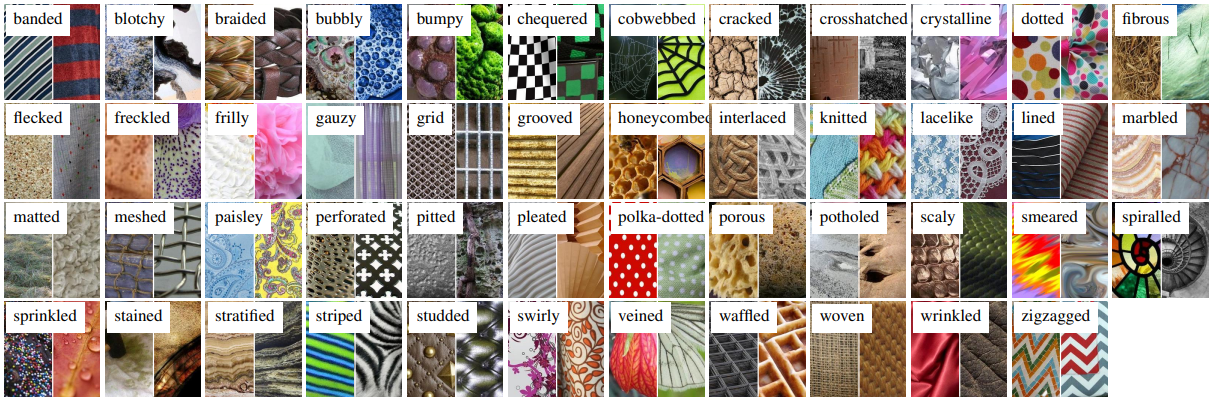
\includegraphics[width=1\textwidth]{assets/images/texturedataset.png}
    \caption{A sample of the describable texture dataset, from
        \citeauthor*{cimpoi_describing_2014} \cite{cimpoi_describing_2014}. }
    \label{fig:texturedataset}
\end{figure}

A visual attribute is a characteristic of an object that is measured visually
and also has some semantic meaning \cite{cimpoi_describing_2014}. For example,
the color of an object is a visual attribute. By categorizing objects based on
their common visual attributes, we can obtain more detailed information about
the relationships between objects. Patterns and textures are important visual
attributes in many applications, such as image processing, pattern recognition,
and computer vision. Analysis of textures can be broken into three main
categories: texture classification, texture segmentation, and texture synthesis
\cite{reed_review_1993}. The process of classifying a texture into a set of
categories and relies on three different approaches. In this paper, we focus on
a \textit{model-based approach} which attempts to extract parameters to reveal
common patterns and use those parameters to automatically distinguish between
different textures \cite{maillard_texture_2003}.

\subsection{Deep Learning}

In the past, automated classification methods depended on human-engineered
feature extraction processes, which tended to not generalize to other domains
\cite{duda_pattern_2001}. More recently, neural networks have been shown to be
able to automatically extract features from input data \cite{arel_deep_2010}.
More specifically, \textit{convolutional neural networks} (CNN) can be applied
to multidimensional data (especially images) and learn high-level features that
can be used to automatically classify data \cite{lecun_gradient_1998}. CNNs have
been around for a few decades currently, but improvements have been made over
recent years which have allowed CNNs to have very good performance on a wide
range of tasks.

\newpage

\subsection{Evaluation}

\subsubsection{Quantitative Metrics}

In estimating the performance of a classification model, we wish to evaluate the
ability of the model to make correct classifications. In order to do so, we
simply count the number of correct and incorrect classifications on a test
dataset. To visualize a summary of the models' performance, we can use a
confusion matrix. A confusion matrix is especially useful in a setting with two
classes, but can also be used in a setting with more than two distinct classes.
An example of a confusion matrix is shown in Figure \ref{fig:matrix}. In a two
class setting, the confusion matrix is a square matrix with four entries. The
columns of the matrix represent the true value of the data, typically as
determined by an expert. The rows of the matrix represent the predicted value of
the data, as determined by the model. Using the confusion matrix, we can derive
several meaningful evaluations of the model's performance.

\begin{figure}[h]
    \centering
    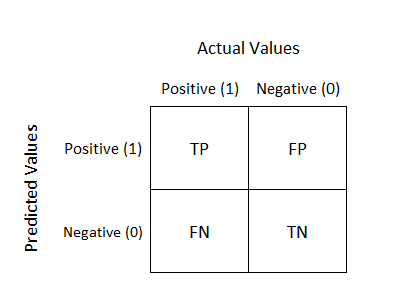
\includegraphics[width=0.5\textwidth]{assets/images/cmatrix.png}
    \caption{Example image of a confusion matrix,
        by \href{https://medium.com/@aatish_kayyath/confusion-matrix-lets-clear-this-confusion-4b0bc5a5983c}{Aatish Kayyath}, is licensed under
        \href{https://creativecommons.org/licenses/by/4.0/}{CC BY 4.0}.}
    \label{fig:matrix}
\end{figure}

\newpage

To begin, we distinguish the following notations:

\begin{itemize}
    \item \textit{True Positive} (TP) - The number of times the model correctly
          classifies a sample as a positive (belonging to the '1' class).
    \item \textit{False Positive} (FP) - The number of times the model incorrectly
          classifies a sample as a positive (belonging to the '1' class).
    \item \textit{True Negative} (TN) - The number of times the model correctly
          classifies a sample as a negative (belonging to the '0' class).
    \item \textit{False Negative} (FN) - The number of times the model incorrectly
          classifies a sample as a negative (belonging to the '0' class).
\end{itemize}

Accuracy is a measure of the correctly classified samples as a percentage of
the total number of samples. The accuracy of a classification model is
calculated as:

\begin{equation}
    \textit{Accuracy} = \frac{TP + TN}{TP + TN + FP + FN}
\end{equation}

Accuracy is a standard evaluation metric for classification models, however, it
can hide the fact that a classification model may be overfitted when the dataset
is imbalanced. We add some other evaluation metrics based on the confusion
matrix.

\newpage
Recall is a measure of the correctly classified samples as a
percentage of the samples that belong to the positive class. The recall of a
classification model is calculated as:

\begin{equation}
    \textit{Recall} = \frac{TP}{TP + FN}
\end{equation}

Recall is typically used in conjuction with the precision. Precision is a
measure of the correctly classified samples as a percentage of the samples that
were predicted to belong to the positive class in addition to the samples that
were actually positive. The precision of a classification model is calculated
as:

\begin{equation}
    \textit{Precision} = \frac{TP}{TP + FP}
\end{equation}

Finally, we examine the F1 score. The F1 score is the harmonic mean of the
precision and recall. The F1 score of a classification model is calculated as:

\begin{equation}
    \textit{F1 Score} = 2 \times \frac{Precision \times Recall}{Precision + Recall}
\end{equation}

\newpage
\subsubsection{Qualitative Metrics}

\begin{figure}[h]
    \centering
    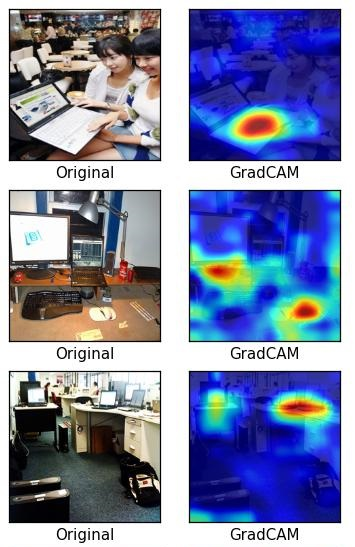
\includegraphics[width=0.5\textwidth]{assets/images/gradcam.jpg}
    \caption{Example image of Grad-CAM applied to images of 'keyboards' from the
        COCO dataset, from \citeauthor*{selvaraju_grad_2020}
        \cite{selvaraju_grad_2020}. }
    \label{fig:gradcam}
\end{figure}

In general, CNN have very good performance on visual recognition tasks. However,
beacuse the learning strategy of a CNN is end-to-end, it is often called a
\textit{black box} - \textit{i.e.} it is difficult to visually interpret the
internal workings of a CNN, yet it is easy to understand the inputs and outputs
\cite{zhang_visual_2018}. One method proposed to produce \textit{visual
    explanations} for CNNs is the \textit{gradient-weighted class activation
    mapping} (Grad-CAM) method \cite{selvaraju_grad_2020}. By using the gradients of
a class from the final convolutional layer, the important regions that lead to
the classification can be identified and visualized. With Grad-CAM, we can
understand the important features learned by the model and how the final
classification was made. Figure \ref{fig:gradcam} shows an example of Grad-CAM
applied to a model that classifies the images of keyboards from the COCO
dataset. The left-side of the figure shows the image that was input to the
model, while the right-side shows the output of Grad-CAM. The heatmap clearly
shows the important features of the image which made the model classify the
image as a keyboard. Applying Grad-CAM will allow us to increase the
interpretability of our models.

\begin{figure}[h]
    \centering
    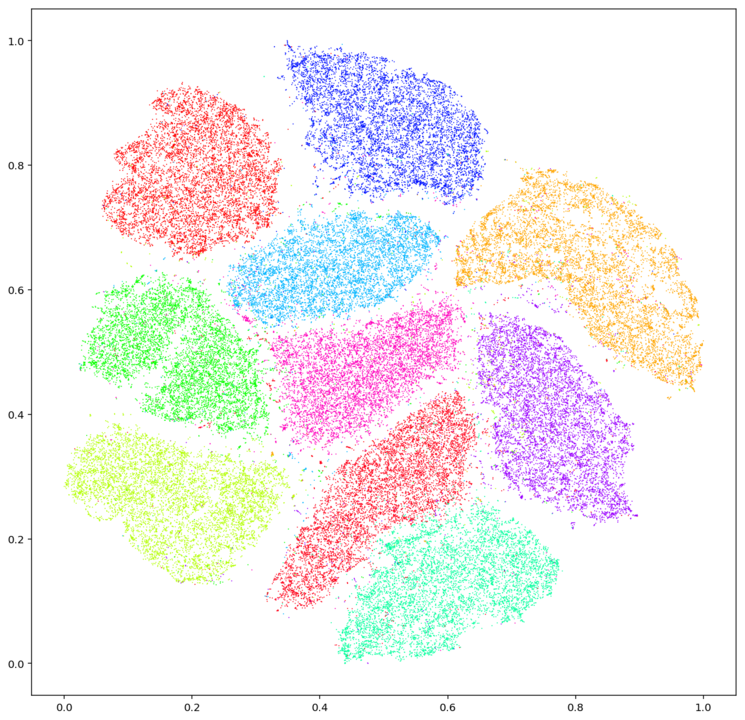
\includegraphics[width=0.7\textwidth]{assets/images/tsne.png}
    \caption{Example image of t-SNE embeddings of MNIST dataset,
        by \href{https://www.flickr.com/photos/kylemcdonald/26620503329/}{Kyle
            McDonald}, is licensed under
        \href{https://creativecommons.org/licenses/by/4.0/}{CC BY 4.0}.}
    \label{fig:tsne}
\end{figure}

For large scale visualization of our data, we must first tackle the
dimensionality of our image dataset. Image data has a large number of dimensions
as a result of each pixel in the image being represented by a tuple of three
values (RGB). \textit{T-distributed stochastic neighbor embedding} (t-SNE) was
proposed for visualizing high-dimensional data in two to three dimensions
\cite{maaten_visualizing_2008}. t-SNE finds similarity between datapoints by
mapping distances into conditional probabilities \cite{maaten_visualizing_2008}.
For an example, the MNIST dataset is a set of images of handwritten digits from
zero to nine, and have a size of 28x28 pixels, for a total of 784 features
\cite{deng_mnist_2012}. An example output embedding of t-SNE on the
MNIST dataset is shown in Figure \ref{fig:tsne}.

\FloatBarrier
\newpage
% ========================================== %
% chapter 3 - literature review
\section{CHAPTER 3: LITERATURE REVIEW}

\begin{figure}[h]
    \centering
    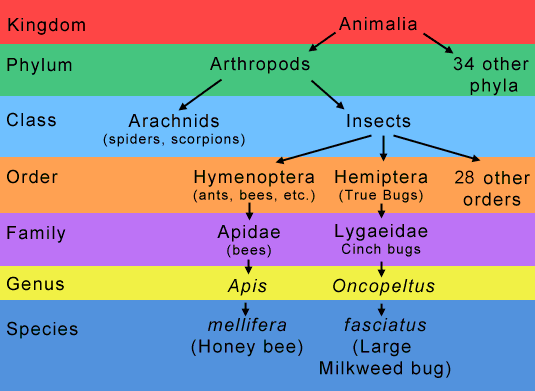
\includegraphics[width=0.6\textwidth]{assets/images/taxonomy-milkweed-bug.png}
    \caption{Taxonomy chart showing taxonomy of the honey bee and large milkweed
        bug. \href{https://askabiologist.asu.edu/sites/default/files/resources/articles/true_bugs/taxomomy-milkweed-bug.gif}{Taxonomy chart}
        by {Adam Dolezal, Page Baluch}, from
        \href{https://askabiologist.asu.edu/explore/true-bugs}{Ask a Biologist}, is licensed under
        \href{https://creativecommons.org/licenses/by/4.0/}{CC BY 4.0}.
    }
    \label{fig:taxonomy-chart}
\end{figure}

\subsection{Insect Classification}

In this section, we provide an overview of some insect classification methods.
Proposed insect classification methods seek to classify insects at different
hierarchical levels, such as species, genus, family, and order. Additionally,
some methods may classify insects at a combination of different hierarchical
levels. An example taxonomy chart with some insect taxonomy is shown in Figure
\ref{fig:taxonomy-chart}. Insect classification methods can be applied to a
variety of fields. In agriculture, insect classification methods can be used to
identify the presence of pest insects in crops, which can inform crop
managers in their choice of pesticides and help prevent crop loss
\cite{liu_pestnet_2019, kasinathan_machine_2021}.

\begin{figure}[h]
    \centering
    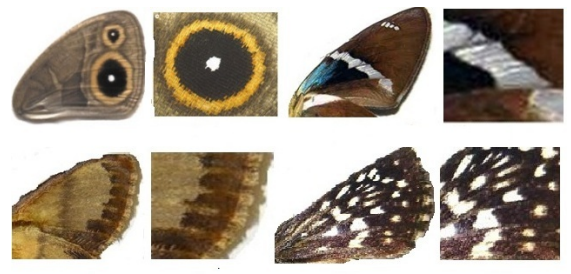
\includegraphics[width=0.8\textwidth]{assets/images/moths.png}
    \caption{An example image of a set of moth wings for moth species
        indentification, from \citeauthor*{feng_automated_2013}
        \cite{feng_automated_2013}.}
    \label{fig:moths}
\end{figure}

\citeauthor*{feng_automated_2013} apply an automated system to classify moth
images based on semantic related visual attributes, which are defined as a
pattern on the moth wings \cite{feng_automated_2013}.
\citeauthor*{feng_automated_2013} use a custom texture descriptor based on the
combination of Grey Level Co-occurence Matrtix and \textit{Scale-Invariant
    Feature Transform} (SIFT) features \cite{gotlieb_texture_1990,
    lowe_distinctive_2004}. The method proposed by \citeauthor*{feng_automated_2013}
is used to classify 50 different moth species across 8 families and is based on
standard texture analysis features \cite{feng_automated_2013}. A set of example
moth wing images is shown in Figure \ref{fig:moths}. The results from
\citeauthor*{feng_automated_2013} suggest that traditional feature extraction
techniques for the semantic visual attributes of the moth wings are
sufficient for training a classifier to classify an image between 10 randomly
selected moth species \cite{feng_automated_2013}.

\begin{figure}[h]
    \centering
    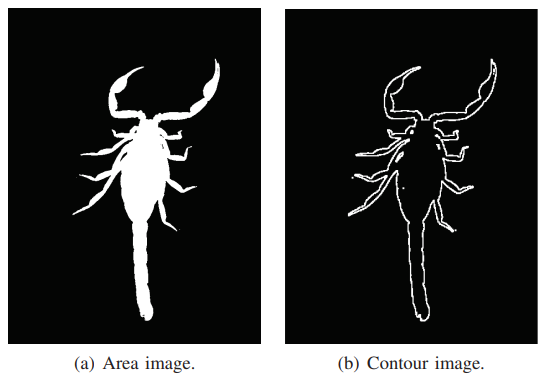
\includegraphics[width=0.8\textwidth]{assets/images/scorpions.png}
    \caption{An example image of a scorpion for a scorpion species classifier
        with the background removed, from \citeauthor*{urteaga_scorpions_2016}
        \cite{urteaga_scorpions_2016}.}
    \label{fig:scorpions}
\end{figure}

\citeauthor*{urteaga_scorpions_2016} use machine learning methods in order to
classify images between two different scorpion species: \textit{Centruroides
    limpidus} and \textit{Centruroides noxius} \cite{urteaga_scorpions_2016}. After
applying background distinction based on dynamic color threshold,
\citeauthor*{urteaga_scorpions_2016} apply feature extraction to extract
features from the separated scorpion image such as aspect ratio, rectangularity,
and compactness \cite{urteaga_scorpions_2016}.
\citeauthor*{urteaga_scorpions_2016} apply three different classification models
to classify the image as one of the species: Artificial Neural Network,
Regression Tree, and Random Forest classifiers \cite{urteaga_scorpions_2016}. An
example image of a scorpion with the background removed is shared in Figure
\ref{fig:scorpions}. The results from \citeauthor*{urteaga_scorpions_2016} show
that after background removal, characteristics from the entire body of the
scorpion can be used to create a binary classifier that can classify the image
as one of the two species. Therefore, we may consider an experiment on the
presence of the background from the ant head image in order to improve
classification accuracy. However, the features extracted from
\cite{urteaga_scorpions_2016} do not make use of any deep learning methods and
are not compatible with our texture-based dataset.
\newpage

\begin{figure}[h]
    \centering
    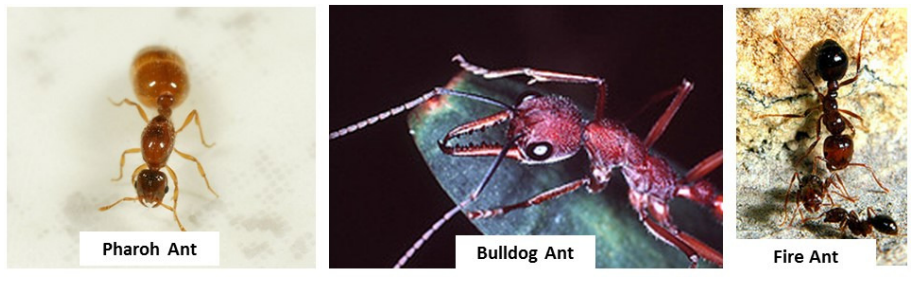
\includegraphics[width=0.8\textwidth]{assets/images/imagenet_ants.png}
    \caption{An example image of three distinct ant species from ImageNet, from
        \citeauthor*{glick_insect_2016} \cite{glick_insect_2016}.}
    \label{fig:imagenet-ants}
\end{figure}

\citeauthor*{lim_performance_2017} apply a CNN-based algorithm for insect
classification \cite{lim_performance_2017}. \citeauthor*{lim_performance_2017}
classify a subset of insect species and families based on the classes available
in the ImageNet dataset \cite{deng_imagenet_2009}. ImageNet is a widely used
dataset of images labeled by experts with millions of images and thousands of
categories \cite{deng_imagenet_2009}. In the ImageNet dataset, there are some
categories that specify the class of the insect on a species level,
\textit{e.g.} \textit{monarch butterfly} and \textit{ringlet butterfly} as well
as some categories that specify the class of the insect on a family level,
\textit{e.g.} \textit{ant}, \textit{fly}, and \textit{bee}
\cite{imagenet_labels}. \citeauthor*{lim_performance_2017} use a modified
AlexNet architecture and experiment with different numbers of kernels and their
effect the performance of the model \cite{lim_performance_2017}.
\citeauthor*{glick_insect_2016} employ a similar approach by classifying 277
insect classes from ImageNet using a hierarchical CNN \cite{glick_insect_2016}.
The results from \citeauthor*{lim_performance_2017} and
\citeauthor*{glick_insect_2016} suggest that a CNN is capable of differentiating
between different hierarchical classes of insects. In our research, we are
interested in the classification of ant images of a hierarchical level between
species and family.

\subsection{Automated Ant Indentification}

In this section, we explore some machine learning methods applied directly to
automated ant systems. We define automated ant systems as methods which process
information about ants in a computer environment. Many automated ant systems
have the purpose of tracking individual ants and their movements. An example of
ant tracking software is shown in Figure \ref{fig:ant-tracking-outdoors}.
Systems that can track multiple individuals in a colony are applied to support
research that investigates social group behaviors of ants
\cite{chandra_foraging_2021, fetter_oxytocin_2021, sclocco_integrating_2020}.

\citeauthor*{sosiak_multidimensional_2021} use morphometric traits as features to
analyze the relationship between the traits and the ecology of the ant
\cite{sosiak_multidimensional_2021}. \citeauthor*{sosiak_multidimensional_2021}
apply a supervised Random Forest algorithm to classify ants based on their
ecology \cite{sosiak_multidimensional_2021}. The research carried out by
\citeauthor*{sosiak_multidimensional_2021} is similar to the end goal of this
research - by creating a system that categorizes ants based on their cuticle
texture, we hope to support a framework that can be used to analyze the
ecological niche of ants in future work.

\begin{figure}[h]
    \centering
    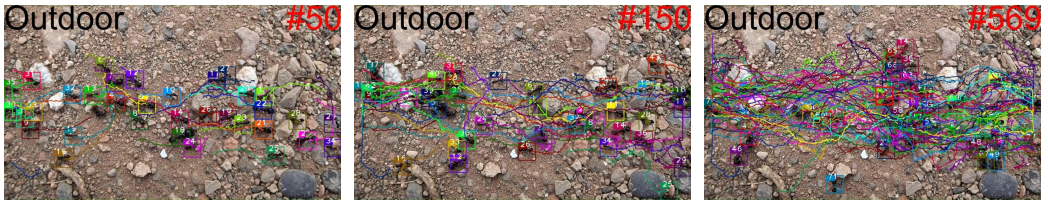
\includegraphics[width=1\textwidth]{assets/images/ant_tracking_outdoors.png}
    \caption{An example output of an individual ant track from a group of
        outdoor ants, from \citeauthor*{cao_online_2020}
        \cite{cao_online_2020}.}
    \label{fig:ant-tracking-outdoors}
\end{figure}

\citeauthor*{cao_online_2020} apply ResNet to automatically extract deep
features from individual ants for offline learning \cite{cao_online_2020}.
\citeauthor*{cao_online_2020} modify the parameters of the softmax classifier to
obtain a cosine similarity metrix classifier to automatically track 10
individual ants in a group \cite{cao_online_2020}. \citeauthor*{cao_online_2020}
use a dataset of 50 images for training and test their model on a much larger
dataset of 24000 images \cite{cao_online_2020}. The results from
\citeauthor*{cao_online_2020} suggest that ResNet is able to differentiate
between individual ants.

\citeauthor*{gal_antrax_2020} also propose a framework for tracking inidividual
insects by taking advantage of color tagging. \citeauthor*{gal_antrax_2020} show
examples of their software tracking individual ants from a group that are
identified with different colors of paint applied to the ants
\cite{gal_antrax_2020}. The method from \citeauthor*{gal_antrax_2020} should
generalize to any type of insect and have relaxed requirements for image quality
due to the constraint of applying color tags \cite{gal_antrax_2020}.  However,
the images of the group of ants used for multi object tracking is not similar to
our dataset of ant head images, other than the fact that both datasets were
collected in a laboratory setting.

\newpage
% ========================================== %
% chapter 4 - methodology
\section{CHAPTER 4: METHODOLOGY}

\subsection{Dataset}

\begin{figure}[h]
    \centering
    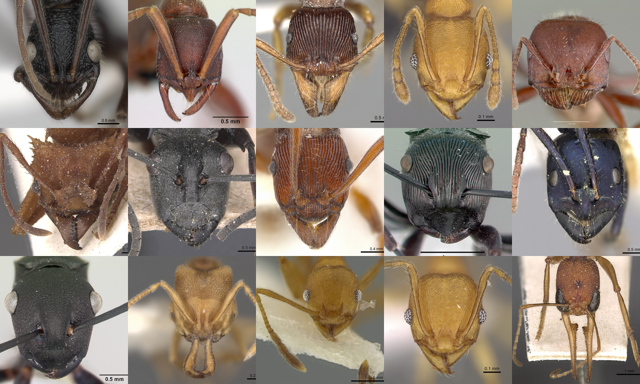
\includegraphics[width=1\textwidth]{assets/images/rough_collage.png}
    \caption{Examples of rough cuticle texture ant images in the dataset after
        center cropping.}
    \label{fig:rough-cuticle-texture}
\end{figure}

In this section, we describe the creation of the custom dataset used in this
research. In our dataset, we classify ant head images from AntWeb
\cite{perrichot_antweb_2012} into two categories: \textit{rough} and
\textit{smooth}. Some randomly selected images from each category are shown in
Figures \ref{fig:rough-cuticle-texture} and \ref{fig:smooth-cuticle-texture}.

\begin{figure}
    \centering
    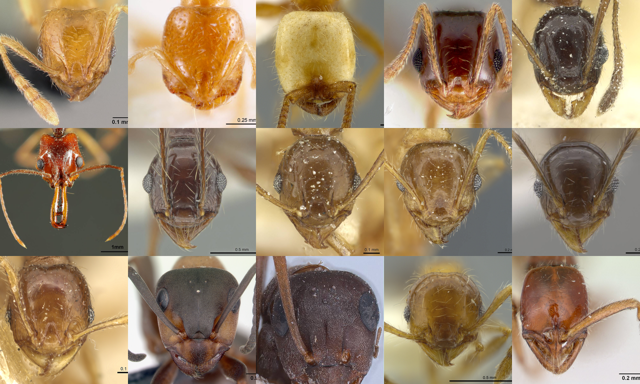
\includegraphics[width=1\textwidth]{assets/images/smooth_collage.png}
    \caption{Examples of smooth cuticle texture ant images in the dataset after
        center cropping.}
    \label{fig:smooth-cuticle-texture}
\end{figure}

\subsubsection{Sculpture Identification Protocol}

To begin, a master spreadsheet was created with the 2,499 different ant species
to be identified for the primary dataset. A team of three assistants were in
charge of the manual identification process. The team was trained to identify
cuticle sculpturing through a process which consisted of one 45-minute
introductory lesson explaining the project and texture categories and then given
a training set of photos to identify from the genus \textit{Polyrhachis}, whose
members display among the highest diversity of cuticle patterns all categories.
The sculpture identification protocol describes the two primary categories:
\textit{rough} and \textit{smooth}.

Initially, the sculpture identification protocol had 8 subcategories of cuticle
texture, including dimpled, ridged, and differing levels of smooth texture. For
simplicity, we work only with the two main categories. The training set
identifications were reviewed together as a group by the assistants. Once
training was complete, assistants were assigned the same genera of ants to
identify independently each week. A weekly meeting was held to discuss
identifications and assign new ones. These identifications were collected in the
master spreadsheet and the identifications were assigned to individual ant
species on a majority basis.

\subsubsection{Data Collection}

To collect the images, the assistants followed the taxonomy information
available in the master spreadsheet to the appropriate AntWeb page. In many
cases, there are multiple ant head images of the same species, and occasionally
there are multiple image resolution available from a single image. To simplify
the data collection process, the assistants were instructed to download the
first ant head image of the species being identified in the highest resolution
possible. Each image was named with an identifier that corresponds with the row
number in the master spreadsheet. The same ant head images that were downloaded
in the data collection phase were the same ones used in the sculpture
identification protocol. Ant species which did not have any images of the head
were excluded from the dataset. Additionally, ant species which only had a head
image of a queen ant were excluded from the dataset.

Ant specimen images taken from AntWeb \cite{perrichot_antweb_2012} are created
by different photographers and therefore have different attributes, such as
environment, resolution, and lighting. In the ant head images, the ant head is
in the center of the image and the body is pointing away from the camera. The
focus of the ant head image is centered on the head, with the background and
image artifacts from the ant body typically blurred. In most ant head images,
there is a bar which indicates the scale of the image due to the variety in the
sizes of different ant species. In a few ant head images, there exists some text
denoting the specimen identifier and other info. In terms of texture, some ant
specimens are very old, so their head images have other abnormalities such as
cracks in the cuticle and the presence of dust.

\subsubsection{Data Preprocessing}

Due to the variety of the ant head image attributes, we apply simple
preprocessing before the images are used in our model. We want the images to
have a uniform size for simplicity in our classification process. Since the ant
head images are typically centered in the image, we apply a center crop to each
image to create a square image of the same size. Once the image is square, we
resize each image to a fixed size of 226x226 pixels. We leave other
discrepancies in the images untouched.

\subsection{Models}
% resnet 
% vgg

\subsection{Evaluation}

We evaluate the performance of the models according to standard evaluation
methods. Since we are working with a binary classification problem, we use a
standard confusion matrix to evaluate the accuracy, precision, and F1 score. We
also apply Grad-CAM with manual inspection to visualize the activation weights
for incorrectly classified images to determine which features are interfering
with the classification. Finally, we apply t-SNE to visualize the seperation
learned for the model to further analyze the classifications made by the model.

\newpage
% ========================================== %
% chapter 5 - experimental results and analysis
\section{CHAPTER 5: EXPERIMENTAL RESULTS AND ANALYSIS}
\subsection{Environment}

\subsection{Results}

\subsection{Analysis}
\newpage
% ========================================== %
% chapter 6 - conclusion
\section{CHAPTER 6: CONCLUSION}

\subsection{Conclusion}

\subsection{Future Work}
\newpage
% ========================================== %
% bibliography
% \setstretch{1} % single spacing
\printbibliography[heading=bibintoc,title={REFERENCES}]
\end{document}
